\documentclass[border=6pt,tikz]{standalone}
\usepackage{tikz}
\usepackage{amsmath,amssymb}
\usetikzlibrary{arrows.meta,positioning,fit,backgrounds,calc,shapes.geometric,decorations.pathreplacing,patterns}
\definecolor{ink}{HTML}{1B2430}
\definecolor{muted}{HTML}{6B7785}
\definecolor{accent}{HTML}{2F6FB5}
\definecolor{accent2}{HTML}{C1611F}
\definecolor{good}{HTML}{2E7D5B}
\definecolor{soft}{HTML}{EDF2F7}
\definecolor{soft2}{HTML}{FBEDE2}
\definecolor{soft3}{HTML}{E6F0E9}
\tikzset{
  box/.style={draw=ink,line width=.7pt,rounded corners=2pt,fill=soft,inner sep=4pt,align=center,font=\sffamily\small},
  boxa/.style={box,fill=soft2},
  boxb/.style={box,fill=soft3},
  plain/.style={align=center,font=\sffamily\small,text=ink},
  tiny/.style={align=center,font=\sffamily\scriptsize,text=muted},
  ar/.style={-{Stealth[length=2.4mm]},draw=ink,line width=.7pt},
  arm/.style={-{Stealth[length=2.4mm]},draw=muted,line width=.6pt,dashed},
  nd/.style={circle,draw=ink,line width=.7pt,fill=white,minimum size=7mm,inner sep=0pt,font=\sffamily\scriptsize},
  ndf/.style={nd,fill=soft},
  ndt/.style={nd,fill=soft2},
}

\begin{document}
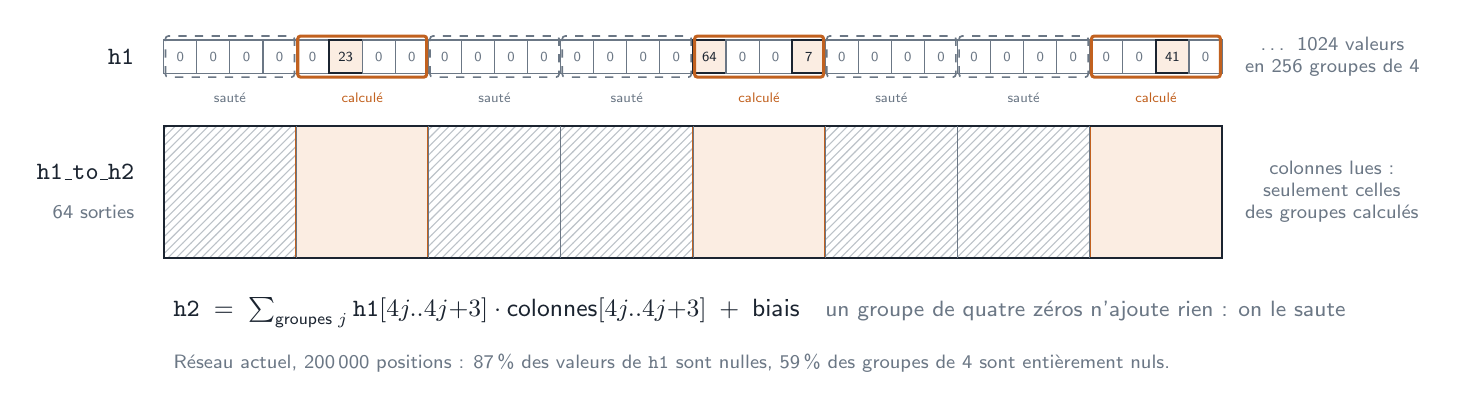
\begin{tikzpicture}[x=4.2mm,y=4.2mm]
  % 32 values of h1 (a window of the 1024), in groups of 4; non-zero values as given below
  \def\vals{0,0,0,0, 0,23,0,0, 0,0,0,0, 0,0,0,0, 64,0,0,7, 0,0,0,0, 0,0,0,0, 0,0,41,0}
  \node[plain,anchor=east] at (-0.6,0.5) {\texttt{h1}};
  \foreach \v [count=\i from 0] in \vals {
    \pgfmathsetmacro{\g}{int(\i/4)}
    \ifnum\v=0
      \draw[muted,line width=.4pt,fill=white] (\i,0) rectangle ++(1,1);
      \node[font=\sffamily\tiny,text=muted] at (\i+.5,.5) {0};
    \else
      \draw[ink,line width=.5pt,fill=soft2] (\i,0) rectangle ++(1,1);
      \node[font=\sffamily\tiny,text=ink] at (\i+.5,.5) {\v};
    \fi
  }
  % group frames
  \foreach \g/\nz in {0/0,1/1,2/0,3/0,4/1,5/0,6/0,7/1} {
    \ifnum\nz=1
      \draw[accent2,line width=1.1pt,rounded corners=1pt] (4*\g+.05,-.12) rectangle ++(3.9,1.24);
      \node[font=\sffamily\tiny,text=accent2] at (4*\g+2,-.75) {calculé};
    \else
      \draw[muted,line width=.6pt,dashed,rounded corners=1pt] (4*\g+.05,-.12) rectangle ++(3.9,1.24);
      \node[font=\sffamily\tiny,text=muted] at (4*\g+2,-.75) {sauté};
    \fi
  }
  \node[tiny,anchor=west] at (32.4,.5) {… 1024 valeurs\\en 256 groupes de 4};
  % the matrix below: 64 rows x the same 32 columns, columns of computed groups shaded
  \begin{scope}[yshift=-23.5mm]
    \node[plain,anchor=east] at (-0.6,2.6) {\texttt{h1\_to\_h2}};
    \node[tiny,anchor=east] at (-0.6,1.4) {64 sorties};
    \foreach \g/\nz in {0/0,1/1,2/0,3/0,4/1,5/0,6/0,7/1} {
      \ifnum\nz=1
        \fill[soft2] (4*\g,0) rectangle ++(4,4);
        \draw[accent2,line width=.8pt] (4*\g,0) rectangle ++(4,4);
      \else
        \fill[pattern=north east lines,pattern color=muted!45] (4*\g,0) rectangle ++(4,4);
      \fi
    }
    \draw[ink,line width=.7pt] (0,0) rectangle (32,4);
    \foreach \x in {4,8,...,28} \draw[muted,line width=.3pt] (\x,0) -- (\x,4);
    \node[tiny,anchor=west] at (32.4,2) {colonnes lues :\\seulement celles\\des groupes calculés};
  \end{scope}
  % formula
  \node[plain,anchor=north west,align=left] at (0,-6.5) {%
    \(\texttt{h2} \;=\; \sum_{\text{groupes } j} \texttt{h1}[4j..4j{+}3] \cdot \text{colonnes}[4j..4j{+}3]
      \;+\; \text{biais}\)\quad
    {\color{muted}\footnotesize un groupe de quatre zéros n'ajoute rien : on le saute}};
  \node[tiny,anchor=north west,align=left] at (0,-8.2) {%
    Réseau actuel, 200\,000 positions : 87\,\% des valeurs de \texttt{h1} sont nulles,
    59\,\% des groupes de 4 sont entièrement nuls.};
\end{tikzpicture}
\end{document}
